\section{Proofs}
\label{app:proofs}

\paragraph{Bayes rule and factorisation.}
For fixed $z$, the conditional risk of $g(z)=a$ is $\mathbb E[e_a\mid z]+\lambda\,\mathbb E[c_0+c_T\mid z]+\lambda\bar c(z)\,a$; the middle term does not depend on $a$, so $a=1$ is strictly better iff $B(z)>\lambda\bar c(z)$, and pointwise minimisation minimises Eq.~(\ref{eq:risk}). If $D=0$, $e_0=e_1$; if $D=1$ and $y\in\{0,1\}$, $e_0=W$ and $e_1=1-W$. Hence $e_0-e_1=D(2W-1)$ and $B(z)=P(D{=}1\mid z)\big(2P(W{=}1\mid D{=}1,z)-1\big)$; for $K$ classes $e_0-e_1=D\big(\mathbf 1[\hat y_1{=}y]-\mathbf 1[\hat y_0{=}y]\big)$ gives $\pi(\rho_1-\rho_0)$. \qed

\paragraph{Proposition~\ref{prop:regret}.}
Where $\hat g(z)\neq g^\star(z)$, the conditional excess risk is $|B-\lambda\bar c|\le|\hat B-B|$, because $\hat B-\lambda\bar c$ and $B-\lambda\bar c$ differ in sign (or $\hat B=\lambda\bar c$). Hence $R(\hat g)-R(g^\star)\le\mathbb E|\hat B-B|$, and $\hat B-B=(\hat\pi-\pi)(2\rho-1)+2\hat\pi(\hat\rho-\rho)$ with the triangle inequality concludes. \qed

\paragraph{Proposition~\ref{prop:efficiency}.}
With $q_i=\sigma(\operatorname{logit}\hat\rho(z_i)+b)$, a labelled target example contributes the log-likelihood $D_i[W_i\log q_i+(1-W_i)\log(1-q_i)]$ (if $D_i=0$, $e_0=e_1$ whatever $y_i$), hence Fisher information $D_i\,q_i(1-q_i)$ about $b$. Its expectation is $P_Q(D{=}1)\,\mathbb E_Q[q(1-q)\mid D{=}1]$ under random sampling and $\mathbb E_Q[q(1-q)\mid D{=}1]$ among disagreements (sampled without labels, as $D$ is observable); information adds over draws. \qed

\section{Disagreement--Advantage Diagnostic Map}
\label{app:diagmap}
\begin{figure}[H]
\begin{minipage}[c]{0.47\textwidth}
% generated by diagnostic_map.py from diagnostic_map.csv; do not edit by hand
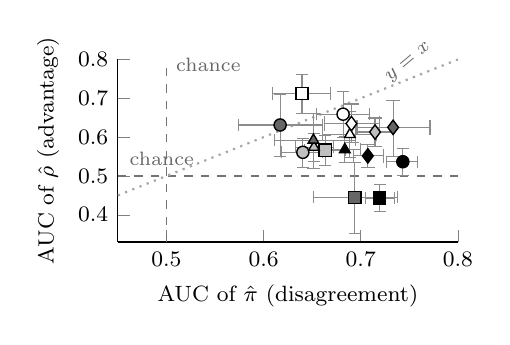
\begin{tikzpicture}
\begin{axis}[width=5.9cm, height=3.9cm, xmin=0.45, xmax=0.80, ymin=0.33, ymax=0.80,
  xlabel={AUC of $\hat\pi$ (disagreement)}, ylabel={AUC of $\hat\rho$ (advantage)},
  label style={font=\footnotesize}, tick label style={font=\footnotesize}, xtick={0.5,0.6,0.7,0.8}, ytick={0.4,0.5,0.6,0.7,0.8},
  axis lines*=left, clip=false, legend cell align=left, 
  error bars/error bar style={black!45, line width=0.4pt}]
\draw[black!55, dashed] (axis cs:0.5,0.33) -- (axis cs:0.5,0.80);
\draw[black!55, dashed] (axis cs:0.45,0.5) -- (axis cs:0.80,0.5);
\draw[black!35, dotted, thick] (axis cs:0.45,0.45) -- (axis cs:0.80,0.80);
\node[font=\scriptsize, text=black!60, anchor=south west] at (axis cs:0.50,0.745) {chance};
\node[font=\scriptsize, text=black!60, anchor=south west] at (axis cs:0.452,0.503) {chance};
\node[font=\scriptsize, text=black!60, rotate=40, anchor=south] at (axis cs:0.76,0.76) {$y=x$};
\addplot[only marks, mark=*, mark size=2.2pt, mark options={draw=black, fill=white, line width=0.5pt}, forget plot, error bars/.cd, x dir=both, x explicit, y dir=both, y explicit] coordinates {(0.6818,0.6591) -= (0.0278,0.0598) += (0.0270,0.0572)};
\addplot[only marks, mark=*, mark size=2.2pt, mark options={draw=black, fill=black!25, line width=0.5pt}, forget plot, error bars/.cd, x dir=both, x explicit, y dir=both, y explicit] coordinates {(0.6404,0.5609) -= (0.0216,0.0385) += (0.0202,0.0349)};
\addplot[only marks, mark=*, mark size=2.2pt, mark options={draw=black, fill=black!60, line width=0.5pt}, forget plot, error bars/.cd, x dir=both, x explicit, y dir=both, y explicit] coordinates {(0.6170,0.6312) -= (0.0426,0.0805) += (0.0432,0.0774)};
\addplot[only marks, mark=*, mark size=2.2pt, mark options={draw=black, fill=black, line width=0.5pt}, forget plot, error bars/.cd, x dir=both, x explicit, y dir=both, y explicit] coordinates {(0.7433,0.5366) -= (0.0169,0.0346) += (0.0153,0.0343)};
\addplot[only marks, mark=square*, mark size=2.2pt, mark options={draw=black, fill=white, line width=0.5pt}, forget plot, error bars/.cd, x dir=both, x explicit, y dir=both, y explicit] coordinates {(0.6395,0.7122) -= (0.0299,0.0506) += (0.0290,0.0493)};
\addplot[only marks, mark=square*, mark size=2.2pt, mark options={draw=black, fill=black!25, line width=0.5pt}, forget plot, error bars/.cd, x dir=both, x explicit, y dir=both, y explicit] coordinates {(0.6634,0.5664) -= (0.0213,0.0392) += (0.0205,0.0385)};
\addplot[only marks, mark=square*, mark size=2.2pt, mark options={draw=black, fill=black!60, line width=0.5pt}, forget plot, error bars/.cd, x dir=both, x explicit, y dir=both, y explicit] coordinates {(0.6938,0.4450) -= (0.0426,0.0935) += (0.0437,0.0898)};
\addplot[only marks, mark=square*, mark size=2.2pt, mark options={draw=black, fill=black, line width=0.5pt}, forget plot, error bars/.cd, x dir=both, x explicit, y dir=both, y explicit] coordinates {(0.7195,0.4431) -= (0.0144,0.0347) += (0.0155,0.0338)};
\addplot[only marks, mark=triangle*, mark size=2.2pt, mark options={draw=black, fill=white, line width=0.5pt}, forget plot, error bars/.cd, x dir=both, x explicit, y dir=both, y explicit] coordinates {(0.6888,0.6068) -= (0.0284,0.0598) += (0.0274,0.0587)};
\addplot[only marks, mark=triangle*, mark size=2.2pt, mark options={draw=black, fill=black!25, line width=0.5pt}, forget plot, error bars/.cd, x dir=both, x explicit, y dir=both, y explicit] coordinates {(0.6518,0.5741) -= (0.0192,0.0361) += (0.0198,0.0362)};
\addplot[only marks, mark=triangle*, mark size=2.2pt, mark options={draw=black, fill=black!60, line width=0.5pt}, forget plot, error bars/.cd, x dir=both, x explicit, y dir=both, y explicit] coordinates {(0.6513,0.5923) -= (0.0403,0.0732) += (0.0433,0.0675)};
\addplot[only marks, mark=triangle*, mark size=2.2pt, mark options={draw=black, fill=black, line width=0.5pt}, forget plot, error bars/.cd, x dir=both, x explicit, y dir=both, y explicit] coordinates {(0.6836,0.5679) -= (0.0162,0.0323) += (0.0158,0.0333)};
\addplot[only marks, mark=diamond*, mark size=2.6pt, mark options={draw=black, fill=white, line width=0.5pt}, forget plot, error bars/.cd, x dir=both, x explicit, y dir=both, y explicit] coordinates {(0.6904,0.6348) -= (0.0278,0.0476) += (0.0285,0.0504)};
\addplot[only marks, mark=diamond*, mark size=2.6pt, mark options={draw=black, fill=black!25, line width=0.5pt}, forget plot, error bars/.cd, x dir=both, x explicit, y dir=both, y explicit] coordinates {(0.7147,0.6131) -= (0.0200,0.0373) += (0.0188,0.0362)};
\addplot[only marks, mark=diamond*, mark size=2.6pt, mark options={draw=black, fill=black!60, line width=0.5pt}, forget plot, error bars/.cd, x dir=both, x explicit, y dir=both, y explicit] coordinates {(0.7333,0.6251) -= (0.0372,0.0760) += (0.0380,0.0696)};
\addplot[only marks, mark=diamond*, mark size=2.6pt, mark options={draw=black, fill=black, line width=0.5pt}, forget plot, error bars/.cd, x dir=both, x explicit, y dir=both, y explicit] coordinates {(0.7073,0.5517) -= (0.0151,0.0293) += (0.0165,0.0286)};
\addlegendimage{only marks, mark=*, mark size=2.2pt, mark options={draw=black, fill=white}}\label{dm:mE5}
\addlegendimage{only marks, mark=square*, mark size=2.2pt, mark options={draw=black, fill=white}}\label{dm:XLMR}
\addlegendimage{only marks, mark=triangle*, mark size=2.2pt, mark options={draw=black, fill=white}}\label{dm:LaBSE}
\addlegendimage{only marks, mark=diamond*, mark size=2.2pt, mark options={draw=black, fill=white}}\label{dm:MARBERTv2}
\addlegendimage{only marks, mark=square*, mark size=2.2pt, mark options={draw=black, fill=white}}\label{dm:S3}
\addlegendimage{only marks, mark=square*, mark size=2.2pt, mark options={draw=black, fill=black!25}}\label{dm:S4}
\addlegendimage{only marks, mark=square*, mark size=2.2pt, mark options={draw=black, fill=black!60}}\label{dm:S5}
\addlegendimage{only marks, mark=square*, mark size=2.2pt, mark options={draw=black, fill=black}}\label{dm:S6}
\end{axis}
\end{tikzpicture}

\end{minipage}\hfill
\begin{minipage}[c]{0.5\textwidth}
\Description{Scatter plot with one point per encoder and test corpus. The x-axis is the AUC of the disagreement estimator, between 0.62 and 0.74 for all points; the y-axis is the AUC of the conditional advantage estimator, mostly between 0.54 and 0.71, with two XLM-R points near 0.44. Dashed lines mark chance at 0.5 on both axes, and a dotted diagonal marks equal AUC. Fourteen of sixteen points lie below the diagonal.}
\caption{Disagreement--advantage diagnostic map (data of Table~\ref{tab:mechanism}; bars: 95\% intervals). Marker: \ref{dm:mE5}\,mE5, \ref{dm:XLMR}\,XLM-R, \ref{dm:LaBSE}\,LaBSE, \ref{dm:MARBERTv2}\,MARBERTv2; fill: \ref{dm:S3}\,$S_3$, \ref{dm:S4}\,$S_4$, \ref{dm:S5}\,$S_5$, \ref{dm:S6}\,$S_6$. $x$: AUC of target-cross-fitted $\hat\pi$ (M1); $y$: AUC of source $\hat\rho$ (M2); dashed: chance; dotted: equal AUC. 14 of 16 points lie below the diagonal; the two near 0.44 are XLM-R on $S_5$ and $S_6$. Linear estimators on $z$ only.}
\label{fig:diagmap}
\end{minipage}
\end{figure}
